\documentclass[12pt]{article}
% REVISION NOTES %%%%%%%%%%%%%%%%%%%%%%%%%%%%%%%%%%%%%%%%%%%%
% 2008-0814 Location, Date, Time
% 2008-0814 fixed citations -- added bibliography.
%
%
\usepackage{geometry}                
\geometry{letterpaper}                   
%\geometry{landscape}                
\usepackage[parfill]{parskip}    
\usepackage{daves,fancyhdr,natbib,graphicx,dcolumn,amsmath,lastpage,url}
\usepackage{amsmath,amssymb,epstopdf,longtable}
\usepackage[final]{pdfpages}
\DeclareGraphicsRule{.tif}{png}{.png}{`convert #1 `dirname #1`/`basename #1 .tif`.png}
\pagestyle{fancy}
\lhead{CE 3305 -- Fluid Mechanics}
\rhead{SPRING 2024}
\lfoot{CE 3305 -- Cleveland}
\cfoot{Page \thepage\ of \pageref{LastPage}}
\rfoot{REVISED: 25 NOV 2023}
\renewcommand\headrulewidth{0pt}
%%%%%%%%%%%%%%%%%%%%%%%%%%%%%%%%%%%%%%%%%%%%%%%%%%%%%%%
\begin{document}
\section*{\center{ { CE 3305 -- Fluid Mechanics} {Exam 1} } }
%\section*{Purpose}
%Demonstrate ability to apply fluid mechanics and problem solving principles covering topics such as: Fluid properties, viscosity, vapor pressure, fluid statics and pressure.
%\section*{Problems}
%\noindent\rule{\linewidth}{0.4pt}
\begin{enumerate}
\item Argon gas is used as a sheilding gas for welding for fabrication of metal objects. A 160-liter tank has an empty weight of 40 kg. \\ \\
Determine:
\begin{enumerate}
\item The total weight of the 160-liter tank of argon at a pressure of 3,500 psia at a temperature of 293$^o$K.  
\end{enumerate}
\noindent\rule{\linewidth}{0.4pt}
\item A fixed mass of water has a bulk modulus of compressibility of $2.2 \times 10^{9} ~Pa$. \\ \\
Determine:
\begin{enumerate}
\item The pressure increase ($\Delta p$) required to reduce the volume of a mass of water by 2-percent (2 \%)
\end{enumerate}
%\noindent\rule{\linewidth}{0.4pt}
%\clearpage
\noindent\rule{\linewidth}{0.4pt}
\item The figure below is a schematic of a sliding plate viscometer used to
measure the viscosity of a fluid. The top plate is moving to the right with a constant
velocity of 10 meters per second in response to a force of 3 Newtons. 

\begin{figure}[htbp] %  figure placement: here, top, bottom, or page
   \centering
   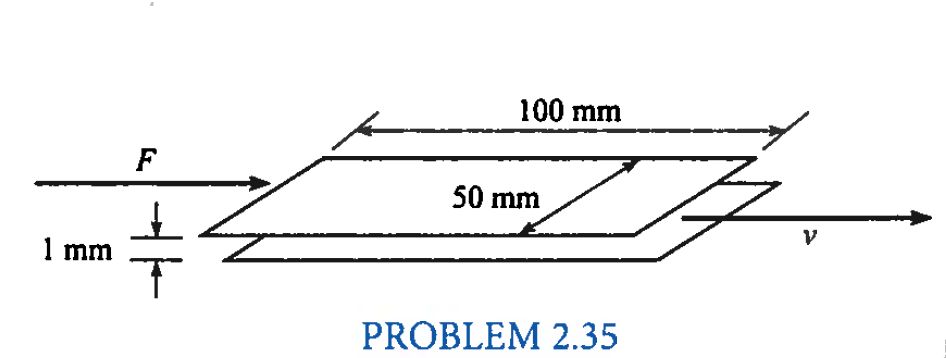
\includegraphics[width=4in]{SlidingPlateViscosity.png} 
   \caption{}
   \label{fig:slidingplateviscosity}
\end{figure}

Determine:
\begin{enumerate}
\item The viscosity of the fluid between the plates.
\end{enumerate}
%\noindent\rule{\linewidth}{0.4pt}
\clearpage
\item A small spherical drop of water with diameter $d=4~mm$  and surface tension ($\sigma = 72.8 \times 10^{-3} \frac{N}{m}$) is depicted in the drawing below.

\begin{figure}[h!] %  figure placement: here, top, bottom, or page
   \centering
   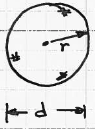
\includegraphics[width=1in]{drop.png} 
   \caption{}
   \label{fig:drop}
\end{figure}

Determine:
\begin{enumerate}
\item The gage pressure of the water in the drop.
\end{enumerate}
%\noindent\rule{\linewidth}{0.4pt}
%\clearpage
\noindent\rule{\linewidth}{0.4pt}
\item A liquid with specific weight of 2700 N/m$^3$ is restrained by a circular gate as ahown.  


\begin{figure}[h!] %  figure placement: here, top, bottom, or page
   \centering
   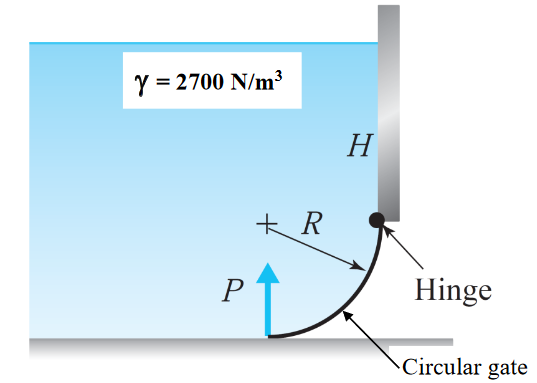
\includegraphics[width=3in]{circlegate.png} 
   \caption{}
   \label{fig:circlegate}
\end{figure}

The dimensions of interest are: R = 1.5 m, H = 6 m, Gate width (into the plane of the image) b = 3 m.

Determine:
\begin{enumerate}
\item The liquid pressure at the hinge.
\item The liquid pressure at the bottom of the gate
\item The horizontal and vertical force of the liquid acting on the circular gate
\end{enumerate}
%\noindent\rule{\linewidth}{0.4pt}
\end{enumerate}
%%%%%%%%%%%%%%%%%%%%%%%%%%%%%%%%%%%%%%%%%%%%%%%%%%%%%%%%%%%%%%%%%%%%%%%%%%%%%%%%%%%%
\bibliographystyle{chicago}	         % (uses file "chicago.bst")
\end{document}


